\documentclass[14pt]{extbook}
\usepackage{multicol, enumerate, enumitem, hyperref, color, soul, setspace, parskip, fancyhdr} %General Packages
\usepackage{amssymb, amsthm, amsmath, bbm, latexsym, units, mathtools} %Math Packages
\everymath{\displaystyle} %All math in Display Style
% Packages with additional options
\usepackage[headsep=0.5cm,headheight=12pt, left=1 in,right= 1 in,top= 1 in,bottom= 1 in]{geometry}
\usepackage[usenames,dvipsnames]{xcolor}
\usepackage{dashrule}  % Package to use the command below to create lines between items
\newcommand{\litem}[1]{\item#1\hspace*{-1cm}\rule{\textwidth}{0.4pt}}
\pagestyle{fancy}
\lhead{Module6}
\chead{}
\rhead{Version A}
\lfoot{9356-6875}
\cfoot{}
\rfoot{testing}
\begin{document}

\begin{enumerate}
\litem{
Describe the end behavior of the polynomial below.\[ f(x) = 8(x - 3)^{4}(x + 3)^{5}(x + 4)^{5}(x - 4)^{5} \]\begin{enumerate}[label=\Alph*.]
\begin{multicols}{2}\item 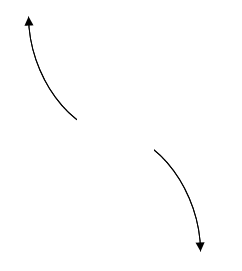
\includegraphics[width = 0.3\textwidth]{../Figures/polyEndBehaviorAA.png}\item 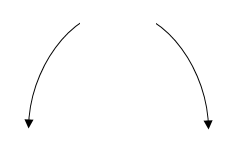
\includegraphics[width = 0.3\textwidth]{../Figures/polyEndBehaviorBA.png}\item 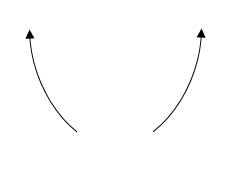
\includegraphics[width = 0.3\textwidth]{../Figures/polyEndBehaviorCA.png}\item 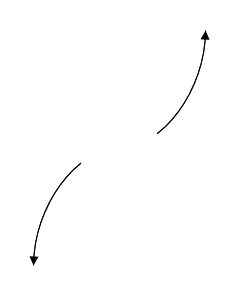
\includegraphics[width = 0.3\textwidth]{../Figures/polyEndBehaviorDA.png}\end{multicols}\item None of the above.
\end{enumerate} }
\litem{
Which of the following equations \textit{could} be of the graph presented below?
\begin{center}
    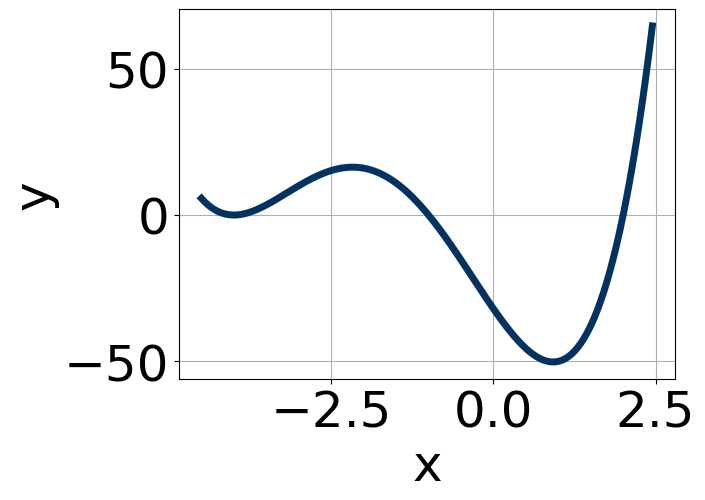
\includegraphics[width=0.5\textwidth]{../Figures/polyGraphToFunctionA.png}
\end{center}
\begin{enumerate}[label=\Alph*.]
\item \( -4(x + 4)^{6} (x - 2)^{9} (x + 1)^{11} \)
\item \( 16(x + 4)^{6} (x - 2)^{4} (x + 1)^{5} \)
\item \( -16(x + 4)^{10} (x - 2)^{11} (x + 1)^{10} \)
\item \( 13(x + 4)^{9} (x - 2)^{8} (x + 1)^{7} \)
\item \( 19(x + 4)^{4} (x - 2)^{7} (x + 1)^{7} \)

\end{enumerate} }
\litem{
Construct the lowest-degree polynomial given the zeros below. Then, choose the intervals that contain the coefficients of the polynomial in the form $ax^3+bx^2+cx+d$.\[ \frac{-2}{3}, \frac{3}{5}, \text{ and } \frac{2}{5} \]\begin{enumerate}[label=\Alph*.]
\item \( a \in [72, 77], b \in [-130, -118], c \in [63, 76], \text{ and } d \in [-16, -11] \)
\item \( a \in [72, 77], b \in [-30, -21], c \in [-35, -29], \text{ and } d \in [9, 15] \)
\item \( a \in [72, 77], b \in [-38, -33], c \in [-30, -21], \text{ and } d \in [9, 15] \)
\item \( a \in [72, 77], b \in [24, 26], c \in [-35, -29], \text{ and } d \in [-16, -11] \)
\item \( a \in [72, 77], b \in [-30, -21], c \in [-35, -29], \text{ and } d \in [-16, -11] \)

\end{enumerate} }
\litem{
Construct the lowest-degree polynomial given the zeros below. Then, choose the intervals that contain the coefficients of the polynomial in the form $x^3+bx^2+cx+d$.\[ -4 - 5 i \text{ and } 1 \]\begin{enumerate}[label=\Alph*.]
\item \( b \in [-11, -2], c \in [30.6, 36.6], \text{ and } d \in [35.9, 45.1] \)
\item \( b \in [0, 5], c \in [3.2, 6.3], \text{ and } d \in [-5.5, -4.6] \)
\item \( b \in [0, 5], c \in [2.1, 3.5], \text{ and } d \in [-4.1, -3.1] \)
\item \( b \in [6, 10], c \in [30.6, 36.6], \text{ and } d \in [-41.6, -37.1] \)
\item \( \text{None of the above.} \)

\end{enumerate} }
\litem{
Construct the lowest-degree polynomial given the zeros below. Then, choose the intervals that contain the coefficients of the polynomial in the form $ax^3+bx^2+cx+d$.\[ 7, -4, \text{ and } \frac{1}{3} \]\begin{enumerate}[label=\Alph*.]
\item \( a \in [-3, 7], b \in [-12, -3], c \in [-85, -77], \text{ and } d \in [25, 30] \)
\item \( a \in [-3, 7], b \in [-12, -3], c \in [-85, -77], \text{ and } d \in [-33, -24] \)
\item \( a \in [-3, 7], b \in [9, 15], c \in [-85, -77], \text{ and } d \in [-33, -24] \)
\item \( a \in [-3, 7], b \in [28, 35], c \in [71, 78], \text{ and } d \in [-33, -24] \)
\item \( a \in [-3, 7], b \in [8, 9], c \in [-89, -86], \text{ and } d \in [25, 30] \)

\end{enumerate} }
\litem{
Construct the lowest-degree polynomial given the zeros below. Then, choose the intervals that contain the coefficients of the polynomial in the form $x^3+bx^2+cx+d$.\[ -2 - 3 i \text{ and } 1 \]\begin{enumerate}[label=\Alph*.]
\item \( b \in [-4.28, -2.11], c \in [7.59, 9.76], \text{ and } d \in [12.72, 14.46] \)
\item \( b \in [0.04, 2.08], c \in [-0.53, 1.89], \text{ and } d \in [-2.5, -1.82] \)
\item \( b \in [2.7, 3.9], c \in [7.59, 9.76], \text{ and } d \in [-13.96, -12.08] \)
\item \( b \in [0.04, 2.08], c \in [1.44, 2.84], \text{ and } d \in [-3.54, -2.67] \)
\item \( \text{None of the above.} \)

\end{enumerate} }
\litem{
Describe the end behavior of the polynomial below.\[ f(x) = 8(x + 4)^{4}(x - 4)^{7}(x - 3)^{4}(x + 3)^{4} \]\begin{enumerate}[label=\Alph*.]
\begin{multicols}{2}\item 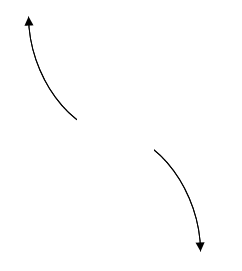
\includegraphics[width = 0.3\textwidth]{../Figures/polyEndBehaviorCopyAA.png}\item 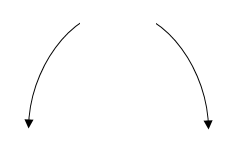
\includegraphics[width = 0.3\textwidth]{../Figures/polyEndBehaviorCopyBA.png}\item 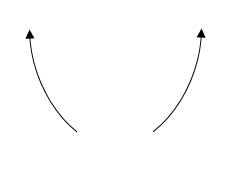
\includegraphics[width = 0.3\textwidth]{../Figures/polyEndBehaviorCopyCA.png}\item 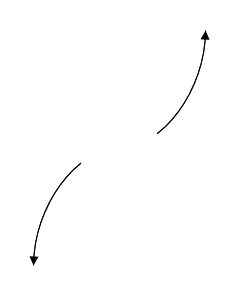
\includegraphics[width = 0.3\textwidth]{../Figures/polyEndBehaviorCopyDA.png}\end{multicols}\item None of the above.
\end{enumerate} }
\litem{
Describe the zero behavior of the zero $x = 7$ of the polynomial below.\[ f(x) = 2(x - 2)^{3}(x + 2)^{2}(x - 7)^{10}(x + 7)^{7} \]\begin{enumerate}[label=\Alph*.]
\begin{multicols}{2}\item 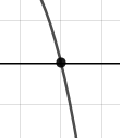
\includegraphics[width = 0.3\textwidth]{../Figures/polyZeroBehaviorAA.png}\item 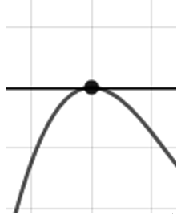
\includegraphics[width = 0.3\textwidth]{../Figures/polyZeroBehaviorBA.png}\item 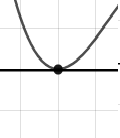
\includegraphics[width = 0.3\textwidth]{../Figures/polyZeroBehaviorCA.png}\item 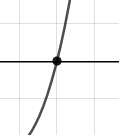
\includegraphics[width = 0.3\textwidth]{../Figures/polyZeroBehaviorDA.png}\end{multicols}\item None of the above.
\end{enumerate} }
\litem{
Describe the zero behavior of the zero $x = 9$ of the polynomial below.\[ f(x) = 2(x + 4)^{13}(x - 4)^{9}(x + 9)^{5}(x - 9)^{4} \]\begin{enumerate}[label=\Alph*.]
\begin{multicols}{2}\item 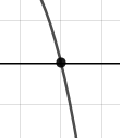
\includegraphics[width = 0.3\textwidth]{../Figures/polyZeroBehaviorCopyAA.png}\item 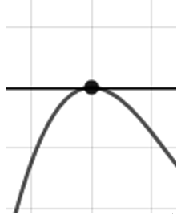
\includegraphics[width = 0.3\textwidth]{../Figures/polyZeroBehaviorCopyBA.png}\item 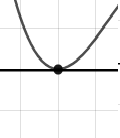
\includegraphics[width = 0.3\textwidth]{../Figures/polyZeroBehaviorCopyCA.png}\item 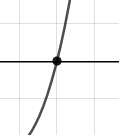
\includegraphics[width = 0.3\textwidth]{../Figures/polyZeroBehaviorCopyDA.png}\end{multicols}\item None of the above.
\end{enumerate} }
\litem{
Which of the following equations \textit{could} be of the graph presented below?
\begin{center}
    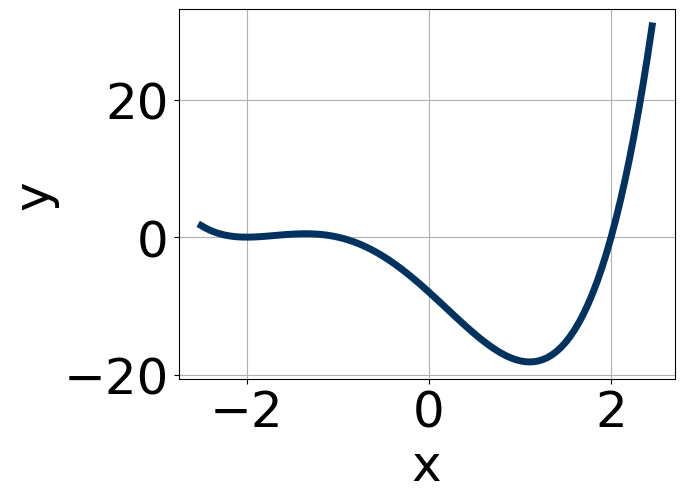
\includegraphics[width=0.5\textwidth]{../Figures/polyGraphToFunctionCopyA.png}
\end{center}
\begin{enumerate}[label=\Alph*.]
\item \( -11(x + 1)^{6} (x + 4)^{11} (x + 3)^{7} \)
\item \( 18(x + 1)^{4} (x + 4)^{10} (x + 3)^{5} \)
\item \( -15(x + 1)^{4} (x + 4)^{6} (x + 3)^{6} \)
\item \( 19(x + 1)^{10} (x + 4)^{4} (x + 3)^{6} \)
\item \( -15(x + 1)^{10} (x + 4)^{6} (x + 3)^{11} \)

\end{enumerate} }
\end{enumerate}

\end{document}